\starthis\section[激光原理]{激光原理} \label{sec:09.05} % 
% \makebox[5em][s]{} % 短题目拉间距

激光是受激辐射的光虽然爱因斯坦早在1917年就提出了原子受激辐射的概念,但在长时期内受激辐射并未得到技术上的应用,因为普通的光源都是利用原子自发辐射,受激辐射虽然同时存在,但其强度远小于自发辐射,微不足道.20世纪50年代出现了微波量子放大器(maser)后,受激辐射受到重视,并很快发明了红宝石激光器(1960 年).从此以后,激光(Laser)在技术应用和理论研究两方面都得到了迅速发展.本节对激光的原理作简单的定性介绍.

回顾$\S$\ref{sec:09.04}讨论过的原子在能级$E_{k}$和$E_{f}$之间的三种跃迁,设$E_{k}<E_{f}$,$E_{k}$称下能级,$E_{f}$称上能级.(为了叙述方便,设$E_{f},E_{k}$是非简并的,每个能级相应于一种定态.)当原子受到$\omega=\omega_{fk}$的光波作用时,处于下能级的原子可以吸收一个光子(能量$\hbar\omega_{fk}$)而跃迁到上能级.处于上能级的原子可以通过自发辐射和受激辐射两种途径向下能级跃迁.原子自发辐射的光是没有方向性的,光子可以向任何方向随机地射出受激辐射的光,其性质(频率,出射方向,偏振性质,相位)与入射光完全相同,这项性质对于激光的形成非常关键,在此稍作解释.电磁场的运动可以按照频率,偏振,运动方向等性质的差别,分解成各种模式的振动(电磁波),光子则是电磁振动的量子化表现.属于同一种振动模式的光子是性质完全相同的玻色子,每种振动模式相当于光子的一种量子态,由于光子是玻色子(自旋为$\hbar$),各个量子态容纳的光子数不受限制.当一个光子射向原子,原子与这种电磁振动模式发生相互作用,原子的能级跃迁就是这种相互作用所引起的.如原子从上能级受激跃迁到下能级,由于能量守恒定律,电磁振动模式将获得能量$(E_{f}-E_{k})$,由于电磁振动是量子化的,其能量变化方式只能是增加一个光子$(\hbar\omega)$.由此可知原子的受激辐射只有当$\omega=\omega_{fk}$才会发生,而辐射的光子与入射光子性质相同.实际上,每种电磁振动模式都存在于整个空间(单色平面波的宽度是无限大),因而同时作用于所有原子,处于下能级的原子可以从中吸收一个光子同时跃迁到上能级.

在通常(热平衡)情况下,原子数按能级的分配遵守玻耳兹曼分布律,下能级原子数远大于上能级原子数,受激辐射的光子数小于被吸收的光子数.如果有办法使上、下能级的原子数分配倒过来,使上能级原子数大大超过下能级原子数,则受激辐射出的光子数大大超过被吸收的光子数,$\omega=\omega_{fk}$电磁振动模式的光子数将迅速增加.由于受激跃迁速率$w_{f\rightarrow k}$与光子数$n(\omega_{fk})$成正比,[\eqref{eq94.12'}式]受激辐射将雪崩式地加速进行,以超过自发辐射的速度在极短时间内使绝大部分处于上能级的原子经由受激辐射而跃迁到下能级,同时获得强度很大的单频辐射光,这就是激光.由于辐射光的光子属于同一种电磁振动模式,所以激光光束有很好的单色性,偏振性和方向性,还有很好的相干性.

制造激光器,首先要找到能够实现上、下能级中原子数分配反转的工作物质其次,建立一个谐振腔,激光管放在腔内(或管、腔合而为一),使受激辐射的光在腔内来回振荡,使它有足够时间去激发其他尚处于上能级的原子,从而造成连锁反应,使受激辐射雪崩式地进行,最终获得强烈的激光输出.谐振腔还有使出射激光谱线宽度变窄,具有良好方向性等作用.

\begin{wrapfigure}[9]{r}{10em}
	\centering
	\small
	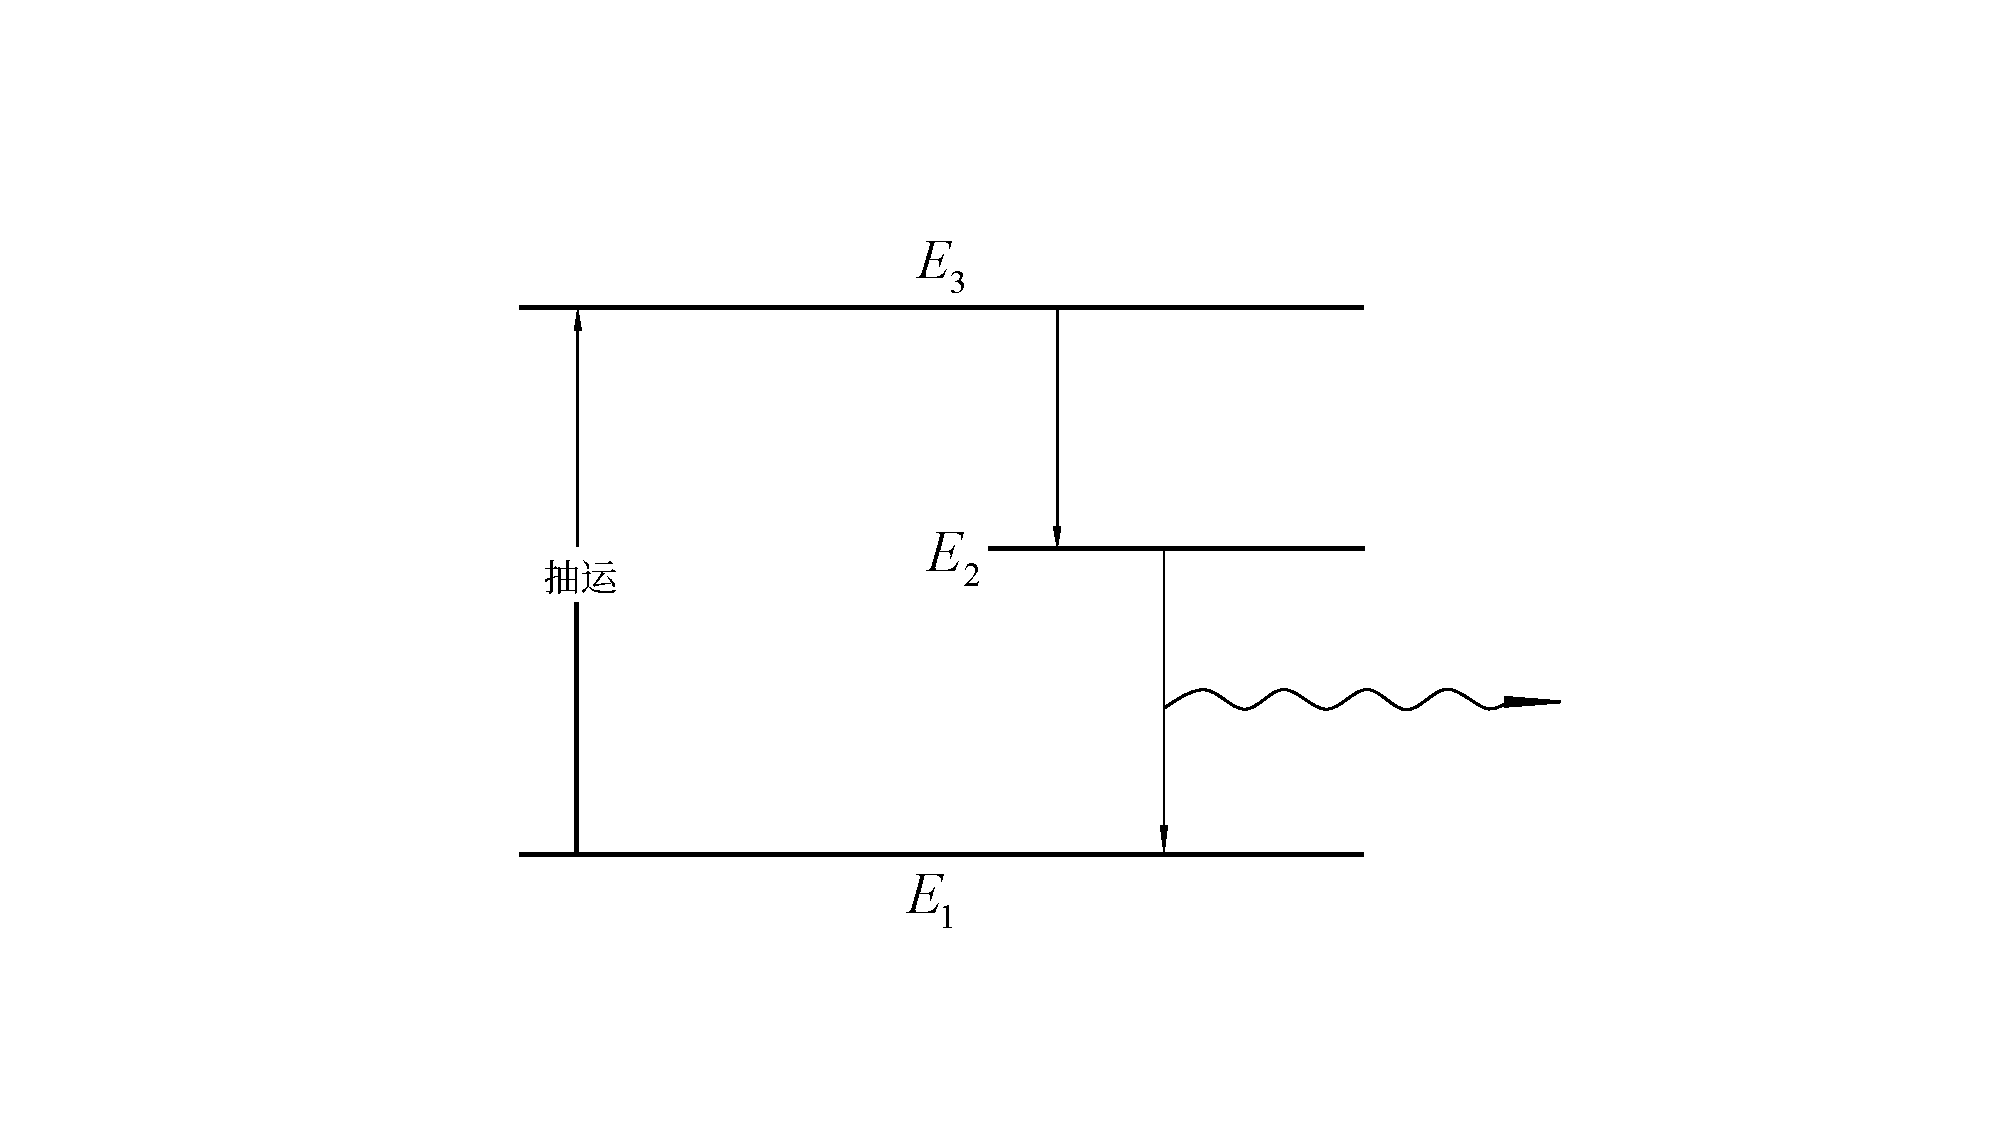
\includegraphics[width=4cm,clip]{QM file/figure/9-3}
	\caption{}\label{fig.9-3}
\end{wrapfigure}
第一代激光器是固体脉冲式,典型代表就是最早出现的红宝石激光器.红宝石是$\ce{Al_{2}O_{3}}$,渗有约0.04\%的\ce{Cr}.利用$\ce{Cr^{+++}}$离子的三能级系统产生激光.这三个能级如图\ref{fig.9-3}所示.用闪光氙灯照射红宝石棒,使$\ce{Cr^{+++}}$从基态能级$E_{1}$上升到$E_{3}$,这个过程称为抽运.$E_{3}$能级经由自发跃迁降到$E_{2}$(寿命约$10^{-7}\si{s}$),$E_{2}$是亚稳态,它与$E_{1}$间的自发跃迁寿命约$10^{-3}\si{s}$.$E_{2}$和$E_{1}$就是用来产生激光的工作能级.如来自氙灯的激发光足够强,在一次闪光时间内$(<10^{-3}\si{s})$就能在上能级$E_{2}$集聚起足够多的$\ce{Cr^{+++}}$离子,实现能级$E_{2}$,$E_{1}$间粒子数反转.红宝石棒的两端面做成平行反射面,(一端有10\%透射率,以获得激光输出)棒本身就是谐振腔.使$E_{2},E_{1}$间产生受激跃迁的最初光讯号就是自发跃迁产生的少数沿棒的轴向传播的光子$(\hbar\omega_{21})$,在两反射面间来回振荡,同时激发更多的$\ce{Cr^{+++}}$离子实现$E_{2}\rightarrow E_{1}$受激辐射,使腔内光讯号迅速放大,成为很强的平行光束,从一端射出这种激光器能量转换(氙灯光能$\rightarrow$激光输出)效率较低,在0.1\%以下.氙灯的每一次闪光,产生一次脉冲式激光(波长\num{694.3}\si{nm})输出,因为是脉冲式,输出激光的单色性并不很好.

能够连续地产生激光,单色性较好的是氦-氖激光器,它利用\ce{Ne}原子的特殊能级构造产生激光,能级图如图\ref{fig.9-4}所示.
\begin{figure}[!h]
	\centering
	\small
	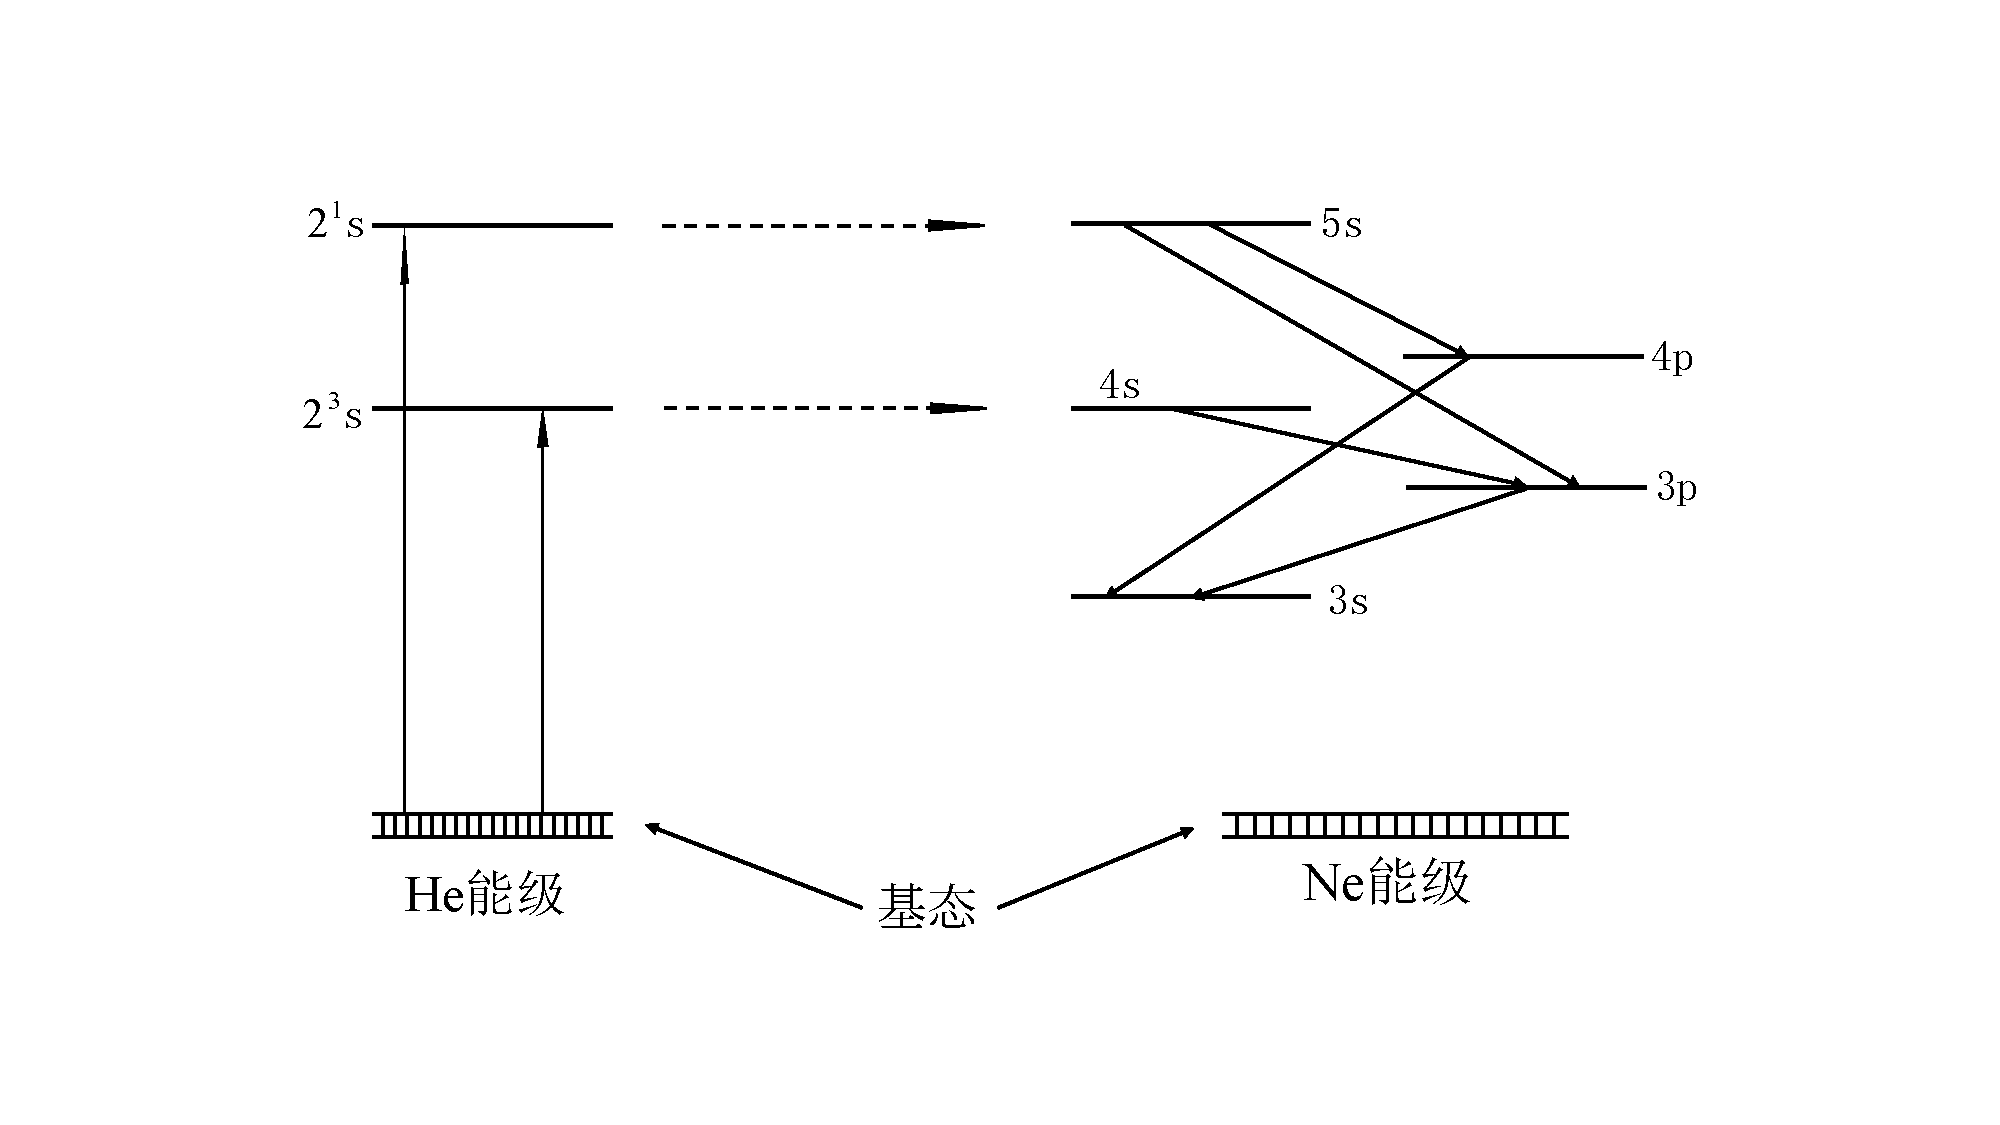
\includegraphics[width=6cm,clip]{QM file/figure/9-4}
	\caption{}\label{fig.9-4}
\end{figure}
\noindent 氦氖激光管中氦与氖约为5:1到10:1,管的两端加上$2\sim3\si{kV}$电压,使产生气体放电,电子的撞击使\ce{He}的一个电子被激发到$2^{1}\si{s}$或$2^{3}\si{s}$能级,再通过气体原子间的碰撞将能量转移给\ce{Ne}原子,使其处于单电子激发能级5s和4s(这两个能级恰好与\ce{He}的$2^{1}\si{s}$及$2^{3}\si{s}$能级接近,容易发生能量转移.)\ce{Ne}原子产生激光的能级跃迁是5s$\rightarrow$4p,5s$\rightarrow$3p,及4s$\rightarrow$3p,由于4p及3p能级原来是空的(\ce{Ne}原子集中在基态能级上),这样就很顺利地实现了上能级与下能级之间的原子数反转.完成受激辐射过程而到达4p及3p能级的原子,可以经由自发跃迁迅速降到3s能级,再经过碰撞降到基态,这样在下能级(4p,3p)就不会积累原子,所以产生激光的过程可以连续进行.造成谐振腔的反射镜可以放在管外,便于调节.氦氖激光有极好的单色性,如\ce{Ne}的5s$\rightarrow$3p跃迁产生的波长\num{632.8}\si{nm}的红光,$\frac{\Delta\nu}{\nu}\sim\num{1.6}\times10^{-11}$.最好的激光$\frac{\Delta\nu}{\nu}$仅$10^{-14}$.

激光器种类很多,发展很快,这里就不多介绍了.
